\documentclass[1p]{elsarticle_modified}
%\bibliographystyle{elsarticle-num}

%\usepackage[colorlinks]{hyperref}
%\usepackage{abbrmath_seonhwa} %\Abb, \Ascr, \Acal ,\Abf, \Afrak
\usepackage{amsfonts}
\usepackage{amssymb}
\usepackage{amsmath}
\usepackage{amsthm}
\usepackage{scalefnt}
\usepackage{amsbsy}
\usepackage{kotex}
\usepackage{caption}
\usepackage{subfig}
\usepackage{color}
\usepackage{graphicx}
\usepackage{xcolor} %% white, black, red, green, blue, cyan, magenta, yellow
\usepackage{float}
\usepackage{setspace}
\usepackage{hyperref}

\usepackage{tikz}
\usetikzlibrary{arrows}

\usepackage{multirow}
\usepackage{array} % fixed length table
\usepackage{hhline}

%%%%%%%%%%%%%%%%%%%%%
\makeatletter
\renewcommand*\env@matrix[1][\arraystretch]{%
	\edef\arraystretch{#1}%
	\hskip -\arraycolsep
	\let\@ifnextchar\new@ifnextchar
	\array{*\c@MaxMatrixCols c}}
\makeatother %https://tex.stackexchange.com/questions/14071/how-can-i-increase-the-line-spacing-in-a-matrix
%%%%%%%%%%%%%%%

\usepackage[normalem]{ulem}

\newcommand{\msout}[1]{\ifmmode\text{\sout{\ensuremath{#1}}}\else\sout{#1}\fi}
%SOURCE: \msout is \stkout macro in https://tex.stackexchange.com/questions/20609/strikeout-in-math-mode

\newcommand{\cancel}[1]{
	\ifmmode
	{\color{red}\msout{#1}}
	\else
	{\color{red}\sout{#1}}
	\fi
}

\newcommand{\add}[1]{
	{\color{blue}\uwave{#1}}
}

\newcommand{\replace}[2]{
	\ifmmode
	{\color{red}\msout{#1}}{\color{blue}\uwave{#2}}
	\else
	{\color{red}\sout{#1}}{\color{blue}\uwave{#2}}
	\fi
}

\newcommand{\Sol}{\mathcal{S}} %segment
\newcommand{\D}{D} %diagram
\newcommand{\A}{\mathcal{A}} %arc


%%%%%%%%%%%%%%%%%%%%%%%%%%%%%5 test

\def\sl{\operatorname{\textup{SL}}(2,\Cbb)}
\def\psl{\operatorname{\textup{PSL}}(2,\Cbb)}
\def\quan{\mkern 1mu \triangleright \mkern 1mu}

\theoremstyle{definition}
\newtheorem{thm}{Theorem}[section]
\newtheorem{prop}[thm]{Proposition}
\newtheorem{lem}[thm]{Lemma}
\newtheorem{ques}[thm]{Question}
\newtheorem{cor}[thm]{Corollary}
\newtheorem{defn}[thm]{Definition}
\newtheorem{exam}[thm]{Example}
\newtheorem{rmk}[thm]{Remark}
\newtheorem{alg}[thm]{Algorithm}

\newcommand{\I}{\sqrt{-1}}
\begin{document}

%\begin{frontmatter}
%
%\title{Boundary parabolic representations of knots up to 8 crossings}
%
%%% Group authors per affiliation:
%\author{Yunhi Cho} 
%\address{Department of Mathematics, University of Seoul, Seoul, Korea}
%\ead{yhcho@uos.ac.kr}
%
%
%\author{Seonhwa Kim} %\fnref{s_kim}}
%\address{Center for Geometry and Physics, Institute for Basic Science, Pohang, 37673, Korea}
%\ead{ryeona17@ibs.re.kr}
%
%\author{Hyuk Kim}
%\address{Department of Mathematical Sciences, Seoul National University, Seoul 08826, Korea}
%\ead{hyukkim@snu.ac.kr}
%
%\author{Seokbeom Yoon}
%\address{Department of Mathematical Sciences, Seoul National University, Seoul, 08826,  Korea}
%\ead{sbyoon15@snu.ac.kr}
%
%\begin{abstract}
%We find all boundary parabolic representation of knots up to 8 crossings.
%
%\end{abstract}
%\begin{keyword}
%    \MSC[2010] 57M25 
%\end{keyword}
%
%\end{frontmatter}

%\linenumbers
%\tableofcontents
%
\newcommand\colored[1]{\textcolor{white}{\rule[-0.35ex]{0.8em}{1.4ex}}\kern-0.8em\color{red} #1}%
%\newcommand\colored[1]{\textcolor{white}{ #1}\kern-2.17ex	\textcolor{white}{ #1}\kern-1.81ex	\textcolor{white}{ #1}\kern-2.15ex\color{red}#1	}

{\Large $\underline{12a_{1254}~(K12a_{1254})}$}

\setlength{\tabcolsep}{10pt}
\renewcommand{\arraystretch}{1.6}
\vspace{1cm}\begin{tabular}{m{100pt}>{\centering\arraybackslash}m{274pt}}
\multirow{5}{120pt}{
	\centering
	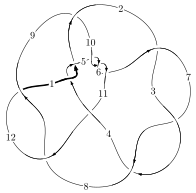
\includegraphics[width=112pt]{../../../GIT/diagram.site/Diagrams/png/2055_12a_1254.png}\\
\ \ \ A knot diagram\footnotemark}&
\allowdisplaybreaks
\textbf{Linearized knot diagam} \\
\cline{2-2}
 &
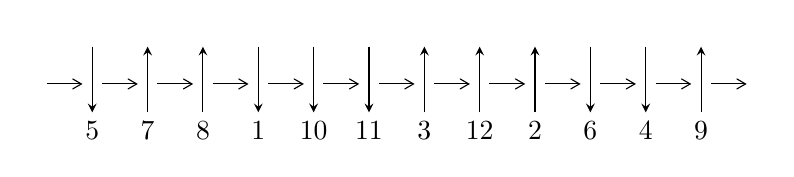
\begin{tikzpicture}[x=20pt, y=17pt]
	% nodes
	\node (C0) at (0, 0) {};
	\node (C1) at (1, 0) {};
	\node (C1U) at (1, +1) {};
	\node (C1D) at (1, -1) {5};

	\node (C2) at (2, 0) {};
	\node (C2U) at (2, +1) {};
	\node (C2D) at (2, -1) {7};

	\node (C3) at (3, 0) {};
	\node (C3U) at (3, +1) {};
	\node (C3D) at (3, -1) {8};

	\node (C4) at (4, 0) {};
	\node (C4U) at (4, +1) {};
	\node (C4D) at (4, -1) {1};

	\node (C5) at (5, 0) {};
	\node (C5U) at (5, +1) {};
	\node (C5D) at (5, -1) {10};

	\node (C6) at (6, 0) {};
	\node (C6U) at (6, +1) {};
	\node (C6D) at (6, -1) {11};

	\node (C7) at (7, 0) {};
	\node (C7U) at (7, +1) {};
	\node (C7D) at (7, -1) {3};

	\node (C8) at (8, 0) {};
	\node (C8U) at (8, +1) {};
	\node (C8D) at (8, -1) {12};

	\node (C9) at (9, 0) {};
	\node (C9U) at (9, +1) {};
	\node (C9D) at (9, -1) {2};

	\node (C10) at (10, 0) {};
	\node (C10U) at (10, +1) {};
	\node (C10D) at (10, -1) {6};

	\node (C11) at (11, 0) {};
	\node (C11U) at (11, +1) {};
	\node (C11D) at (11, -1) {4};

	\node (C12) at (12, 0) {};
	\node (C12U) at (12, +1) {};
	\node (C12D) at (12, -1) {9};
	\node (C13) at (13, 0) {};

	% arrows
	\draw[->,>={angle 60}]
	(C0) edge (C1) (C1) edge (C2) (C2) edge (C3) (C3) edge (C4) (C4) edge (C5) (C5) edge (C6) (C6) edge (C7) (C7) edge (C8) (C8) edge (C9) (C9) edge (C10) (C10) edge (C11) (C11) edge (C12) (C12) edge (C13) ;	\draw[->,>=stealth]
	(C1U) edge (C1D) (C2D) edge (C2U) (C3D) edge (C3U) (C4U) edge (C4D) (C5U) edge (C5D) (C6U) edge (C6D) (C7D) edge (C7U) (C8D) edge (C8U) (C9D) edge (C9U) (C10U) edge (C10D) (C11U) edge (C11D) (C12D) edge (C12U) ;
	\end{tikzpicture} \\
\hhline{~~} \\& 
\textbf{Solving Sequence} \\ \cline{2-2} 
 &
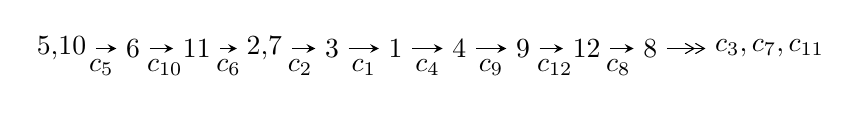
\begin{tikzpicture}[x=23pt, y=7pt]
	% node
	\node (A0) at (-1/8, 0) {5,10};
	\node (A1) at (1, 0) {6};
	\node (A2) at (2, 0) {11};
	\node (A3) at (49/16, 0) {2,7};
	\node (A4) at (33/8, 0) {3};
	\node (A5) at (41/8, 0) {1};
	\node (A6) at (49/8, 0) {4};
	\node (A7) at (57/8, 0) {9};
	\node (A8) at (65/8, 0) {12};
	\node (A9) at (73/8, 0) {8};
	\node (C1) at (1/2, -1) {$c_{5}$};
	\node (C2) at (3/2, -1) {$c_{10}$};
	\node (C3) at (5/2, -1) {$c_{6}$};
	\node (C4) at (29/8, -1) {$c_{2}$};
	\node (C5) at (37/8, -1) {$c_{1}$};
	\node (C6) at (45/8, -1) {$c_{4}$};
	\node (C7) at (53/8, -1) {$c_{9}$};
	\node (C8) at (61/8, -1) {$c_{12}$};
	\node (C9) at (69/8, -1) {$c_{8}$};
	\node (A10) at (11, 0) {$c_{3},c_{7},c_{11}$};

	% edge
	\draw[->,>=stealth]	
	(A0) edge (A1) (A1) edge (A2) (A2) edge (A3) (A3) edge (A4) (A4) edge (A5) (A5) edge (A6) (A6) edge (A7) (A7) edge (A8) (A8) edge (A9) ;
	\draw[->>,>={angle 60}]	
	(A9) edge (A10);
\end{tikzpicture} \\ 

\end{tabular} \\

\footnotetext{
The image of knot diagram is generated by the software ``\textbf{Draw programme}" developed by Andrew Bartholomew(\url{http://www.layer8.co.uk/maths/draw/index.htm\#Running-draw}), where we modified some parts for our purpose(\url{https://github.com/CATsTAILs/LinksPainter}).
}\phantom \\ \newline 
\centering \textbf{Ideals for irreducible components\footnotemark of $X_{\text{par}}$} 
 
\begin{align*}
I^u_{1}&=\langle 
-1.63090\times10^{126} u^{71}-1.43198\times10^{127} u^{70}+\cdots+1.61786\times10^{128} b+1.62123\times10^{128},\\
\phantom{I^u_{1}}&\phantom{= \langle  }-1.10105\times10^{130} u^{71}-3.48895\times10^{130} u^{70}+\cdots+3.39751\times10^{129} a+5.30987\times10^{130},\\
\phantom{I^u_{1}}&\phantom{= \langle  }u^{72}+3 u^{71}+\cdots-26 u^2+1\rangle \\
\\
\end{align*}
\raggedright * 1 irreducible components of $\dim_{\mathbb{C}}=0$, with total 72 representations.\\
\footnotetext{All coefficients of polynomials are rational numbers. But the coefficients are sometimes approximated in decimal forms when there is not enough margin.}
\newpage
\renewcommand{\arraystretch}{1}
\centering \section*{I. $I^u_{1}= \langle -1.63\times10^{126} u^{71}-1.43\times10^{127} u^{70}+\cdots+1.62\times10^{128} b+1.62\times10^{128},\;-1.10\times10^{130} u^{71}-3.49\times10^{130} u^{70}+\cdots+3.40\times10^{129} a+5.31\times10^{130},\;u^{72}+3 u^{71}+\cdots-26 u^2+1 \rangle$}
\flushleft \textbf{(i) Arc colorings}\\
\begin{tabular}{m{7pt} m{180pt} m{7pt} m{180pt} }
\flushright $a_{5}=$&$\begin{pmatrix}1\\0\end{pmatrix}$ \\
\flushright $a_{10}=$&$\begin{pmatrix}0\\u\end{pmatrix}$ \\
\flushright $a_{6}=$&$\begin{pmatrix}1\\u^2\end{pmatrix}$ \\
\flushright $a_{11}=$&$\begin{pmatrix}- u\\- u^3+u\end{pmatrix}$ \\
\flushright $a_{2}=$&$\begin{pmatrix}3.24076 u^{71}+10.2691 u^{70}+\cdots-136.064 u-15.6287\\0.0100806 u^{71}+0.0885108 u^{70}+\cdots+0.154524 u-1.00208\end{pmatrix}$ \\
\flushright $a_{7}=$&$\begin{pmatrix}- u^2+1\\- u^4+2 u^2\end{pmatrix}$ \\
\flushright $a_{3}=$&$\begin{pmatrix}3.01036 u^{71}+9.56914 u^{70}+\cdots-129.487 u-15.8619\\0.0443474 u^{71}+0.191702 u^{70}+\cdots+0.547558 u-0.927506\end{pmatrix}$ \\
\flushright $a_{1}=$&$\begin{pmatrix}3.25084 u^{71}+10.3576 u^{70}+\cdots-135.909 u-16.6308\\0.0100806 u^{71}+0.0885108 u^{70}+\cdots+0.154524 u-1.00208\end{pmatrix}$ \\
\flushright $a_{4}=$&$\begin{pmatrix}3.93995 u^{71}+12.1793 u^{70}+\cdots-144.274 u-18.1963\\-0.205083 u^{71}-0.696225 u^{70}+\cdots-1.51684 u-0.931392\end{pmatrix}$ \\
\flushright $a_{9}=$&$\begin{pmatrix}25.0206 u^{71}+79.2187 u^{70}+\cdots-1012.78 u-151.398\\0.440428 u^{71}+1.31089 u^{70}+\cdots-17.2649 u-4.14504\end{pmatrix}$ \\
\flushright $a_{12}=$&$\begin{pmatrix}28.8160 u^{71}+90.4805 u^{70}+\cdots-1156.38 u-175.392\\0.437569 u^{71}+1.27882 u^{70}+\cdots-21.8953 u-4.40858\end{pmatrix}$ \\
\flushright $a_{8}=$&$\begin{pmatrix}-3.44954 u^{71}-11.3202 u^{70}+\cdots+159.467 u+31.2821\\-0.193079 u^{71}-0.610090 u^{70}+\cdots+6.79834 u-0.0918382\end{pmatrix}$\\&\end{tabular}
\flushleft \textbf{(ii) Obstruction class $= -1$}\\~\\
\flushleft \textbf{(iii) Cusp Shapes $= 5.04864 u^{71}+17.1634 u^{70}+\cdots-197.061 u-30.2965$}\\~\\
\newpage\renewcommand{\arraystretch}{1}
\flushleft \textbf{(iv) u-Polynomials at the component}\newline \\
\begin{tabular}{m{50pt}|m{274pt}}
Crossings & \hspace{64pt}u-Polynomials at each crossing \\
\hline $$\begin{aligned}c_{1},c_{4}\end{aligned}$$&$\begin{aligned}
&u^{72}+u^{71}+\cdots-16 u+1
\end{aligned}$\\
\hline $$\begin{aligned}c_{2},c_{3},c_{7}\end{aligned}$$&$\begin{aligned}
&u^{72}+3 u^{71}+\cdots-26 u^2+1
\end{aligned}$\\
\hline $$\begin{aligned}c_{5},c_{6},c_{10}\end{aligned}$$&$\begin{aligned}
&u^{72}-3 u^{71}+\cdots-26 u^2+1
\end{aligned}$\\
\hline $$\begin{aligned}c_{8},c_{12}\end{aligned}$$&$\begin{aligned}
&u^{72}- u^{71}+\cdots+16 u+1
\end{aligned}$\\
\hline $$\begin{aligned}c_{9}\end{aligned}$$&$\begin{aligned}
&63(63 u^{72}+1197 u^{71}+\cdots-137930 u-101308)
\end{aligned}$\\
\hline $$\begin{aligned}c_{11}\end{aligned}$$&$\begin{aligned}
&63(63 u^{72}-1197 u^{71}+\cdots+137930 u-101308)
\end{aligned}$\\
\hline
\end{tabular}\\~\\
\newpage\renewcommand{\arraystretch}{1}
\flushleft \textbf{(v) Riley Polynomials at the component}\newline \\
\begin{tabular}{m{50pt}|m{274pt}}
Crossings & \hspace{64pt}Riley Polynomials at each crossing \\
\hline $$\begin{aligned}c_{1},c_{4},c_{8}\\c_{12}\end{aligned}$$&$\begin{aligned}
&y^{72}-51 y^{71}+\cdots-20 y+1
\end{aligned}$\\
\hline $$\begin{aligned}c_{2},c_{3},c_{5}\\c_{6},c_{7},c_{10}\end{aligned}$$&$\begin{aligned}
&y^{72}-71 y^{71}+\cdots-52 y+1
\end{aligned}$\\
\hline $$\begin{aligned}c_{9},c_{11}\end{aligned}$$&$\begin{aligned}
&3969\\
&\cdot(3969 y^{72}-532791 y^{71}+\cdots+24968314100 y+10263310864)
\end{aligned}$\\
\hline
\end{tabular}\\~\\
\newpage\flushleft \textbf{(vi) Complex Volumes and Cusp Shapes}
$$\begin{array}{c|c|c}  
\text{Solutions to }I^u_{1}& \I (\text{vol} + \sqrt{-1}CS) & \text{Cusp shape}\\
 \hline 
\begin{aligned}
u &= \phantom{-}0.649955 + 0.767013 I \\
a &= \phantom{-}0.371690 + 0.863674 I \\
b &= -1.157260 - 0.177201 I\end{aligned}
 & -3.51621 - 2.84598 I & \phantom{-0.000000 } 0 \\ \hline\begin{aligned}
u &= \phantom{-}0.649955 - 0.767013 I \\
a &= \phantom{-}0.371690 - 0.863674 I \\
b &= -1.157260 + 0.177201 I\end{aligned}
 & -3.51621 + 2.84598 I & \phantom{-0.000000 } 0 \\ \hline\begin{aligned}
u &= \phantom{-}0.755046 + 0.607683 I \\
a &= \phantom{-}0.958639 - 0.782753 I \\
b &= \phantom{-}0.211107 + 0.677137 I\end{aligned}
 & \phantom{-}9.48984 + 1.78690 I & \phantom{-0.000000 } 0 \\ \hline\begin{aligned}
u &= \phantom{-}0.755046 - 0.607683 I \\
a &= \phantom{-}0.958639 + 0.782753 I \\
b &= \phantom{-}0.211107 - 0.677137 I\end{aligned}
 & \phantom{-}9.48984 - 1.78690 I & \phantom{-0.000000 } 0 \\ \hline\begin{aligned}
u &= \phantom{-}0.561764 + 0.889787 I \\
a &= -0.343337 - 1.311210 I \\
b &= \phantom{-}1.285200 + 0.503327 I\end{aligned}
 & \phantom{-}6.85180 - 11.78730 I & \phantom{-0.000000 } 0 \\ \hline\begin{aligned}
u &= \phantom{-}0.561764 - 0.889787 I \\
a &= -0.343337 + 1.311210 I \\
b &= \phantom{-}1.285200 - 0.503327 I\end{aligned}
 & \phantom{-}6.85180 + 11.78730 I & \phantom{-0.000000 } 0 \\ \hline\begin{aligned}
u &= -0.566060 + 0.689487 I \\
a &= \phantom{-}0.38171 - 1.40245 I \\
b &= -1.258670 + 0.517373 I\end{aligned}
 & \phantom{-0.000000 -}8.38473 I & \phantom{-0.000000 } 0 \\ \hline\begin{aligned}
u &= -0.566060 - 0.689487 I \\
a &= \phantom{-}0.38171 + 1.40245 I \\
b &= -1.258670 - 0.517373 I\end{aligned}
 & \phantom{-0.000000 } -8.38473 I & \phantom{-0.000000 } 0 \\ \hline\begin{aligned}
u &= -0.401846 + 0.784856 I \\
a &= \phantom{-}0.911206 - 0.151398 I \\
b &= -1.075360 - 0.313339 I\end{aligned}
 & \phantom{-}0.50187 - 3.59150 I & \phantom{-0.000000 -}0. + 6.84899 I \\ \hline\begin{aligned}
u &= -0.401846 - 0.784856 I \\
a &= \phantom{-}0.911206 + 0.151398 I \\
b &= -1.075360 + 0.313339 I\end{aligned}
 & \phantom{-}0.50187 + 3.59150 I & \phantom{-0.000000 } 0. - 6.84899 I\\
 \hline 
 \end{array}$$\newpage$$\begin{array}{c|c|c}  
\text{Solutions to }I^u_{1}& \I (\text{vol} + \sqrt{-1}CS) & \text{Cusp shape}\\
 \hline 
\begin{aligned}
u &= \phantom{-}0.360230 + 0.755264 I \\
a &= -0.121619 + 1.340780 I \\
b &= \phantom{-}0.060046 - 1.002070 I\end{aligned}
 & \phantom{-}10.66310 - 6.45840 I & \phantom{-}7.25218 + 5.11414 I \\ \hline\begin{aligned}
u &= \phantom{-}0.360230 - 0.755264 I \\
a &= -0.121619 - 1.340780 I \\
b &= \phantom{-}0.060046 + 1.002070 I\end{aligned}
 & \phantom{-}10.66310 + 6.45840 I & \phantom{-}7.25218 - 5.11414 I \\ \hline\begin{aligned}
u &= \phantom{-}0.649376 + 0.994071 I \\
a &= -0.537633 + 0.012831 I \\
b &= \phantom{-}1.131150 - 0.361477 I\end{aligned}
 & \phantom{-}6.71683 + 5.69927 I & \phantom{-0.000000 } 0 \\ \hline\begin{aligned}
u &= \phantom{-}0.649376 - 0.994071 I \\
a &= -0.537633 - 0.012831 I \\
b &= \phantom{-}1.131150 + 0.361477 I\end{aligned}
 & \phantom{-}6.71683 - 5.69927 I & \phantom{-0.000000 } 0 \\ \hline\begin{aligned}
u &= -0.474762 + 1.140520 I \\
a &= -0.524061 + 0.650730 I \\
b &= \phantom{-}1.171890 - 0.205962 I\end{aligned}
 & \phantom{-}1.64587 + 4.92294 I & \phantom{-0.000000 } 0 \\ \hline\begin{aligned}
u &= -0.474762 - 1.140520 I \\
a &= -0.524061 - 0.650730 I \\
b &= \phantom{-}1.171890 + 0.205962 I\end{aligned}
 & \phantom{-}1.64587 - 4.92294 I & \phantom{-0.000000 } 0 \\ \hline\begin{aligned}
u &= -0.208137 + 0.704884 I \\
a &= \phantom{-}0.708628 - 1.104090 I \\
b &= -0.091169 + 0.449600 I\end{aligned}
 & \phantom{-}5.21021 + 2.48118 I & \phantom{-}6.35115 - 4.16718 I \\ \hline\begin{aligned}
u &= -0.208137 - 0.704884 I \\
a &= \phantom{-}0.708628 + 1.104090 I \\
b &= -0.091169 - 0.449600 I\end{aligned}
 & \phantom{-}5.21021 - 2.48118 I & \phantom{-}6.35115 + 4.16718 I \\ \hline\begin{aligned}
u &= -1.267630 + 0.242344 I \\
a &= \phantom{-}0.752454 - 0.638834 I \\
b &= -0.101250 + 0.346802 I\end{aligned}
 & \phantom{-}2.11200 + 1.03313 I & \phantom{-0.000000 } 0 \\ \hline\begin{aligned}
u &= -1.267630 - 0.242344 I \\
a &= \phantom{-}0.752454 + 0.638834 I \\
b &= -0.101250 - 0.346802 I\end{aligned}
 & \phantom{-}2.11200 - 1.03313 I & \phantom{-0.000000 } 0\\
 \hline 
 \end{array}$$\newpage$$\begin{array}{c|c|c}  
\text{Solutions to }I^u_{1}& \I (\text{vol} + \sqrt{-1}CS) & \text{Cusp shape}\\
 \hline 
\begin{aligned}
u &= \phantom{-}1.32452\phantom{ +0.000000I} \\
a &= -0.890875\phantom{ +0.000000I} \\
b &= -2.07992\phantom{ +0.000000I}\end{aligned}
 & \phantom{-}2.49962\phantom{ +0.000000I} & \phantom{-0.000000 } 0 \\ \hline\begin{aligned}
u &= -1.346220 + 0.078526 I \\
a &= -0.291387 + 0.201598 I \\
b &= -1.38956 - 1.17852 I\end{aligned}
 & \phantom{-}1.46224 + 2.61815 I & \phantom{-0.000000 } 0 \\ \hline\begin{aligned}
u &= -1.346220 - 0.078526 I \\
a &= -0.291387 - 0.201598 I \\
b &= -1.38956 + 1.17852 I\end{aligned}
 & \phantom{-}1.46224 - 2.61815 I & \phantom{-0.000000 } 0 \\ \hline\begin{aligned}
u &= \phantom{-}1.363600 + 0.025152 I \\
a &= -0.513667 - 0.148824 I \\
b &= -0.113437 + 0.094897 I\end{aligned}
 & -3.19701 - 0.01303 I & \phantom{-0.000000 } 0 \\ \hline\begin{aligned}
u &= \phantom{-}1.363600 - 0.025152 I \\
a &= -0.513667 + 0.148824 I \\
b &= -0.113437 - 0.094897 I\end{aligned}
 & -3.19701 + 0.01303 I & \phantom{-0.000000 } 0 \\ \hline\begin{aligned}
u &= -1.37923\phantom{ +0.000000I} \\
a &= -1.92010\phantom{ +0.000000I} \\
b &= -1.32845\phantom{ +0.000000I}\end{aligned}
 & -1.08828\phantom{ +0.000000I} & \phantom{-0.000000 } 0 \\ \hline\begin{aligned}
u &= \phantom{-}0.434671 + 0.429294 I \\
a &= -0.56763 - 1.50065 I \\
b &= \phantom{-}1.215410 + 0.596589 I\end{aligned}
 & -0.50187 - 3.59150 I & -0.30026 + 6.84899 I \\ \hline\begin{aligned}
u &= \phantom{-}0.434671 - 0.429294 I \\
a &= -0.56763 + 1.50065 I \\
b &= \phantom{-}1.215410 - 0.596589 I\end{aligned}
 & -0.50187 + 3.59150 I & -0.30026 - 6.84899 I \\ \hline\begin{aligned}
u &= \phantom{-}1.388510 + 0.125096 I \\
a &= \phantom{-}0.295480 - 0.465640 I \\
b &= \phantom{-}0.27946 + 1.49621 I\end{aligned}
 & -1.64587 - 4.92294 I & \phantom{-0.000000 } 0 \\ \hline\begin{aligned}
u &= \phantom{-}1.388510 - 0.125096 I \\
a &= \phantom{-}0.295480 + 0.465640 I \\
b &= \phantom{-}0.27946 - 1.49621 I\end{aligned}
 & -1.64587 + 4.92294 I & \phantom{-0.000000 } 0\\
 \hline 
 \end{array}$$\newpage$$\begin{array}{c|c|c}  
\text{Solutions to }I^u_{1}& \I (\text{vol} + \sqrt{-1}CS) & \text{Cusp shape}\\
 \hline 
\begin{aligned}
u &= \phantom{-}1.398290 + 0.071099 I \\
a &= \phantom{-}0.058738 - 0.776258 I \\
b &= -0.912296 + 0.581047 I\end{aligned}
 & -2.11200 - 1.03313 I & \phantom{-0.000000 } 0 \\ \hline\begin{aligned}
u &= \phantom{-}1.398290 - 0.071099 I \\
a &= \phantom{-}0.058738 + 0.776258 I \\
b &= -0.912296 - 0.581047 I\end{aligned}
 & -2.11200 + 1.03313 I & \phantom{-0.000000 } 0 \\ \hline\begin{aligned}
u &= -0.551714 + 0.218194 I \\
a &= \phantom{-}0.121797 + 0.972740 I \\
b &= \phantom{-}1.181600 - 0.138253 I\end{aligned}
 & -2.64681 + 0.31493 I & -3.09974 + 2.98415 I \\ \hline\begin{aligned}
u &= -0.551714 - 0.218194 I \\
a &= \phantom{-}0.121797 - 0.972740 I \\
b &= \phantom{-}1.181600 + 0.138253 I\end{aligned}
 & -2.64681 - 0.31493 I & -3.09974 - 2.98415 I \\ \hline\begin{aligned}
u &= -1.404890 + 0.097683 I \\
a &= \phantom{-}0.063758 + 0.734444 I \\
b &= \phantom{-}0.395294 - 0.764529 I\end{aligned}
 & -5.21021 + 2.48118 I & \phantom{-0.000000 } 0 \\ \hline\begin{aligned}
u &= -1.404890 - 0.097683 I \\
a &= \phantom{-}0.063758 - 0.734444 I \\
b &= \phantom{-}0.395294 + 0.764529 I\end{aligned}
 & -5.21021 - 2.48118 I & \phantom{-0.000000 } 0 \\ \hline\begin{aligned}
u &= \phantom{-}1.40558 + 0.24747 I \\
a &= -0.083482 + 0.851271 I \\
b &= -0.216127 - 0.825464 I\end{aligned}
 & \phantom{-0.000000 } -5.89665 I & \phantom{-0.000000 } 0 \\ \hline\begin{aligned}
u &= \phantom{-}1.40558 - 0.24747 I \\
a &= -0.083482 - 0.851271 I \\
b &= -0.216127 + 0.825464 I\end{aligned}
 & \phantom{-0.000000 -}5.89665 I & \phantom{-0.000000 } 0 \\ \hline\begin{aligned}
u &= -0.501776 + 0.266487 I \\
a &= -1.68326 - 0.64048 I \\
b &= -0.349712 + 0.435136 I\end{aligned}
 & \phantom{-}2.64681 - 0.31493 I & \phantom{-}3.09974 - 2.98415 I \\ \hline\begin{aligned}
u &= -0.501776 - 0.266487 I \\
a &= -1.68326 + 0.64048 I \\
b &= -0.349712 - 0.435136 I\end{aligned}
 & \phantom{-}2.64681 + 0.31493 I & \phantom{-}3.09974 + 2.98415 I\\
 \hline 
 \end{array}$$\newpage$$\begin{array}{c|c|c}  
\text{Solutions to }I^u_{1}& \I (\text{vol} + \sqrt{-1}CS) & \text{Cusp shape}\\
 \hline 
\begin{aligned}
u &= -1.44069\phantom{ +0.000000I} \\
a &= \phantom{-}6.02414\phantom{ +0.000000I} \\
b &= \phantom{-}1.02295\phantom{ +0.000000I}\end{aligned}
 & -4.98750\phantom{ +0.000000I} & \phantom{-0.000000 } 0 \\ \hline\begin{aligned}
u &= -1.44554 + 0.26940 I \\
a &= -0.382483 - 0.613995 I \\
b &= -0.139489 + 1.196830 I\end{aligned}
 & \phantom{-}4.86838 + 10.14510 I & \phantom{-0.000000 } 0 \\ \hline\begin{aligned}
u &= -1.44554 - 0.26940 I \\
a &= -0.382483 + 0.613995 I \\
b &= -0.139489 - 1.196830 I\end{aligned}
 & \phantom{-}4.86838 - 10.14510 I & \phantom{-0.000000 } 0 \\ \hline\begin{aligned}
u &= -0.246051 + 0.465180 I \\
a &= \phantom{-}0.19086 + 1.49758 I \\
b &= -0.139532 - 1.090770 I\end{aligned}
 & \phantom{-}3.51621 + 2.84598 I & \phantom{-}7.08728 - 8.53827 I \\ \hline\begin{aligned}
u &= -0.246051 - 0.465180 I \\
a &= \phantom{-}0.19086 - 1.49758 I \\
b &= -0.139532 + 1.090770 I\end{aligned}
 & \phantom{-}3.51621 - 2.84598 I & \phantom{-}7.08728 + 8.53827 I \\ \hline\begin{aligned}
u &= -1.47163 + 0.14528 I \\
a &= \phantom{-}0.565549 + 0.814669 I \\
b &= \phantom{-}1.57798 - 0.67208 I\end{aligned}
 & -6.71683 + 5.69927 I & \phantom{-0.000000 } 0 \\ \hline\begin{aligned}
u &= -1.47163 - 0.14528 I \\
a &= \phantom{-}0.565549 - 0.814669 I \\
b &= \phantom{-}1.57798 + 0.67208 I\end{aligned}
 & -6.71683 - 5.69927 I & \phantom{-0.000000 } 0 \\ \hline\begin{aligned}
u &= \phantom{-}1.51164 + 0.11669 I \\
a &= \phantom{-}0.684539 - 0.713923 I \\
b &= \phantom{-}1.44150 + 0.28466 I\end{aligned}
 & -9.48984 - 1.78690 I & \phantom{-0.000000 } 0 \\ \hline\begin{aligned}
u &= \phantom{-}1.51164 - 0.11669 I \\
a &= \phantom{-}0.684539 + 0.713923 I \\
b &= \phantom{-}1.44150 - 0.28466 I\end{aligned}
 & -9.48984 + 1.78690 I & \phantom{-0.000000 } 0 \\ \hline\begin{aligned}
u &= \phantom{-}0.227486 + 0.392172 I \\
a &= -2.91334 - 1.86372 I \\
b &= \phantom{-}0.976660 - 0.216723 I\end{aligned}
 & \phantom{-0.000000 -}0.906236 I & \phantom{-0.000000 -}0. + 9.31169 I\\
 \hline 
 \end{array}$$\newpage$$\begin{array}{c|c|c}  
\text{Solutions to }I^u_{1}& \I (\text{vol} + \sqrt{-1}CS) & \text{Cusp shape}\\
 \hline 
\begin{aligned}
u &= \phantom{-}0.227486 - 0.392172 I \\
a &= -2.91334 + 1.86372 I \\
b &= \phantom{-}0.976660 + 0.216723 I\end{aligned}
 & \phantom{-0.000000 } -0.906236 I & \phantom{-0.000000 } 0. - 9.31169 I \\ \hline\begin{aligned}
u &= \phantom{-}1.53124 + 0.23600 I \\
a &= -0.569957 + 1.044770 I \\
b &= -1.46206 - 0.58160 I\end{aligned}
 & -6.85180 - 11.78730 I & \phantom{-0.000000 } 0 \\ \hline\begin{aligned}
u &= \phantom{-}1.53124 - 0.23600 I \\
a &= -0.569957 - 1.044770 I \\
b &= -1.46206 + 0.58160 I\end{aligned}
 & -6.85180 + 11.78730 I & \phantom{-0.000000 } 0 \\ \hline\begin{aligned}
u &= -1.55559\phantom{ +0.000000I} \\
a &= \phantom{-}1.08766\phantom{ +0.000000I} \\
b &= -0.193111\phantom{ +0.000000I}\end{aligned}
 & \phantom{-}1.08828\phantom{ +0.000000I} & \phantom{-0.000000 } 0 \\ \hline\begin{aligned}
u &= -1.54857 + 0.24062 I \\
a &= -0.476741 - 0.923449 I \\
b &= -1.38209 + 0.33972 I\end{aligned}
 & -10.66310 + 6.45840 I & \phantom{-0.000000 } 0 \\ \hline\begin{aligned}
u &= -1.54857 - 0.24062 I \\
a &= -0.476741 + 0.923449 I \\
b &= -1.38209 - 0.33972 I\end{aligned}
 & -10.66310 - 6.45840 I & \phantom{-0.000000 } 0 \\ \hline\begin{aligned}
u &= \phantom{-}0.216451 + 0.368593 I \\
a &= -0.516118 - 0.919730 I \\
b &= \phantom{-}0.122854 + 0.327294 I\end{aligned}
 & \phantom{-0.000000 } -0.846056 I & \phantom{-0.000000 -}0. + 8.06993 I \\ \hline\begin{aligned}
u &= \phantom{-}0.216451 - 0.368593 I \\
a &= -0.516118 + 0.919730 I \\
b &= \phantom{-}0.122854 - 0.327294 I\end{aligned}
 & \phantom{-0.000000 -}0.846056 I & \phantom{-0.000000 } 0. - 8.06993 I \\ \hline\begin{aligned}
u &= -1.55377 + 0.31543 I \\
a &= \phantom{-}0.587127 + 1.178050 I \\
b &= \phantom{-}1.42437 - 0.53718 I\end{aligned}
 & \phantom{-0.000000 -}16.1961 I & \phantom{-0.000000 } 0 \\ \hline\begin{aligned}
u &= -1.55377 - 0.31543 I \\
a &= \phantom{-}0.587127 - 1.178050 I \\
b &= \phantom{-}1.42437 + 0.53718 I\end{aligned}
 & \phantom{-0.000000 } -16.1961 I & \phantom{-0.000000 } 0\\
 \hline 
 \end{array}$$\newpage$$\begin{array}{c|c|c}  
\text{Solutions to }I^u_{1}& \I (\text{vol} + \sqrt{-1}CS) & \text{Cusp shape}\\
 \hline 
\begin{aligned}
u &= \phantom{-}1.54410 + 0.36847 I \\
a &= \phantom{-}0.336253 - 1.043030 I \\
b &= \phantom{-}1.350500 + 0.365176 I\end{aligned}
 & -4.86838 - 10.14510 I & \phantom{-0.000000 } 0 \\ \hline\begin{aligned}
u &= \phantom{-}1.54410 - 0.36847 I \\
a &= \phantom{-}0.336253 + 1.043030 I \\
b &= \phantom{-}1.350500 - 0.365176 I\end{aligned}
 & -4.86838 + 10.14510 I & \phantom{-0.000000 } 0 \\ \hline\begin{aligned}
u &= \phantom{-}0.104562 + 0.393865 I \\
a &= \phantom{-}0.765029 - 1.020030 I \\
b &= -1.49104 + 0.54161 I\end{aligned}
 & \phantom{-}5.95339 - 0.98579 I & \phantom{-}13.4814 + 6.1699 I \\ \hline\begin{aligned}
u &= \phantom{-}0.104562 - 0.393865 I \\
a &= \phantom{-}0.765029 + 1.020030 I \\
b &= -1.49104 - 0.54161 I\end{aligned}
 & \phantom{-}5.95339 + 0.98579 I & \phantom{-}13.4814 - 6.1699 I \\ \hline\begin{aligned}
u &= \phantom{-}1.62235 + 0.28986 I \\
a &= -0.362610 + 0.552302 I \\
b &= -1.131580 - 0.066438 I\end{aligned}
 & -5.95339 - 0.98579 I & \phantom{-0.000000 } 0 \\ \hline\begin{aligned}
u &= \phantom{-}1.62235 - 0.28986 I \\
a &= -0.362610 - 0.552302 I \\
b &= -1.131580 + 0.066438 I\end{aligned}
 & -5.95339 + 0.98579 I & \phantom{-0.000000 } 0 \\ \hline\begin{aligned}
u &= -1.55311 + 0.67597 I \\
a &= -0.002070 + 0.554887 I \\
b &= \phantom{-}1.171780 - 0.109704 I\end{aligned}
 & -1.46224 + 2.61815 I & \phantom{-0.000000 } 0 \\ \hline\begin{aligned}
u &= -1.55311 - 0.67597 I \\
a &= -0.002070 - 0.554887 I \\
b &= \phantom{-}1.171780 + 0.109704 I\end{aligned}
 & -1.46224 - 2.61815 I & \phantom{-0.000000 } 0 \\ \hline\begin{aligned}
u &= -0.258714 + 0.094467 I \\
a &= \phantom{-}3.50898 + 1.82058 I \\
b &= -0.846426 - 0.103474 I\end{aligned}
 & \phantom{-}3.19701 + 0.01303 I & \phantom{-}0.976771 + 0.960819 I \\ \hline\begin{aligned}
u &= -0.258714 - 0.094467 I \\
a &= \phantom{-}3.50898 - 1.82058 I \\
b &= -0.846426 + 0.103474 I\end{aligned}
 & \phantom{-}3.19701 - 0.01303 I & \phantom{-}0.976771 - 0.960819 I\\
 \hline 
 \end{array}$$\newpage$$\begin{array}{c|c|c}  
\text{Solutions to }I^u_{1}& \I (\text{vol} + \sqrt{-1}CS) & \text{Cusp shape}\\
 \hline 
\begin{aligned}
u &= \phantom{-}0.155044\phantom{ +0.000000I} \\
a &= -52.3313\phantom{ +0.000000I} \\
b &= -1.07077\phantom{ +0.000000I}\end{aligned}
 & \phantom{-}4.98750\phantom{ +0.000000I} & -83.9270\phantom{ +0.000000I} \\ \hline\begin{aligned}
u &= -1.95291\phantom{ +0.000000I} \\
a &= \phantom{-}0.284351\phantom{ +0.000000I} \\
b &= \phantom{-}1.16979\phantom{ +0.000000I}\end{aligned}
 & -2.49962\phantom{ +0.000000I} & \phantom{-0.000000 } 0\\
 \hline 
 \end{array}$$\newpage
\newpage\renewcommand{\arraystretch}{1}
\centering \section*{ II. u-Polynomials}
\begin{tabular}{m{50pt}|m{274pt}}
Crossings & \hspace{64pt}u-Polynomials at each crossing \\
\hline $$\begin{aligned}c_{1},c_{4}\end{aligned}$$&$\begin{aligned}
&u^{72}+u^{71}+\cdots-16 u+1
\end{aligned}$\\
\hline $$\begin{aligned}c_{2},c_{3},c_{7}\end{aligned}$$&$\begin{aligned}
&u^{72}+3 u^{71}+\cdots-26 u^2+1
\end{aligned}$\\
\hline $$\begin{aligned}c_{5},c_{6},c_{10}\end{aligned}$$&$\begin{aligned}
&u^{72}-3 u^{71}+\cdots-26 u^2+1
\end{aligned}$\\
\hline $$\begin{aligned}c_{8},c_{12}\end{aligned}$$&$\begin{aligned}
&u^{72}- u^{71}+\cdots+16 u+1
\end{aligned}$\\
\hline $$\begin{aligned}c_{9}\end{aligned}$$&$\begin{aligned}
&63(63 u^{72}+1197 u^{71}+\cdots-137930 u-101308)
\end{aligned}$\\
\hline $$\begin{aligned}c_{11}\end{aligned}$$&$\begin{aligned}
&63(63 u^{72}-1197 u^{71}+\cdots+137930 u-101308)
\end{aligned}$\\
\hline
\end{tabular}\newpage\renewcommand{\arraystretch}{1}
\centering \section*{ III. Riley Polynomials}
\begin{tabular}{m{50pt}|m{274pt}}
Crossings & \hspace{64pt}Riley Polynomials at each crossing \\
\hline $$\begin{aligned}c_{1},c_{4},c_{8}\\c_{12}\end{aligned}$$&$\begin{aligned}
&y^{72}-51 y^{71}+\cdots-20 y+1
\end{aligned}$\\
\hline $$\begin{aligned}c_{2},c_{3},c_{5}\\c_{6},c_{7},c_{10}\end{aligned}$$&$\begin{aligned}
&y^{72}-71 y^{71}+\cdots-52 y+1
\end{aligned}$\\
\hline $$\begin{aligned}c_{9},c_{11}\end{aligned}$$&$\begin{aligned}
&3969\\
&\cdot(3969 y^{72}-532791 y^{71}+\cdots+24968314100 y+10263310864)
\end{aligned}$\\
\hline
\end{tabular}
\vskip 2pc
\end{document}